\documentclass[tikz]{standalone}
\usepackage{tikz}
\usepackage{graphicx}

\usetikzlibrary{calc, angles, quotes}
\usetikzlibrary{intersections} % Necessário para achar pontos de cruzamento

%\newfontfamily\gotham{Gotham-Black}
%\newfontfamily\cambria{Cambria}

\begin{document}

\begin{tikzpicture}
    \node[scale=2] at (0,0) {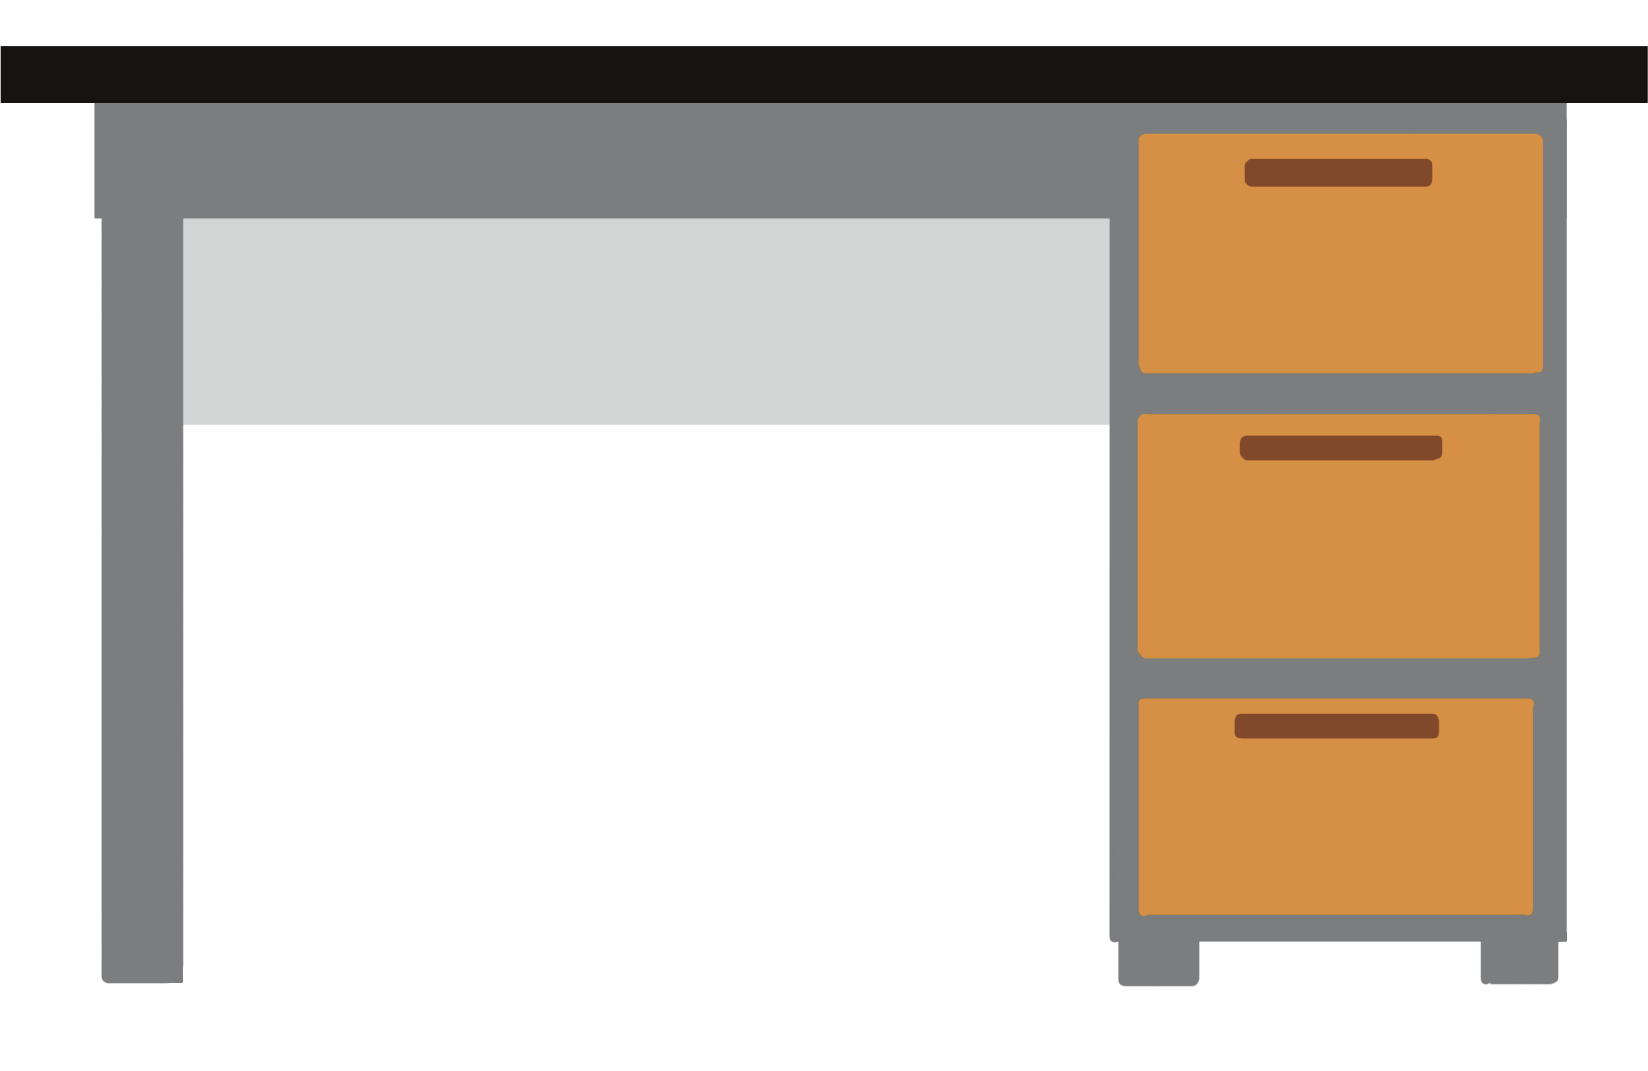
\includegraphics[width=0.25\textwidth]{Simulado_3-atividade_4.png}}; 
    \node[fill=red!40,rounded corners] at (0,2.7) {Mesa para escritório};
    \node at (0,2.2) {$R\$ 400,00$};
    \node[fill=red!40,rounded corners] at (0,-2.3) {E nas compras à vista};
    \node at (0,-2.8) {desconto de $25\%$};    
\end{tikzpicture}
\end{document}